\documentclass[11pt]{article}

% Packages
\usepackage[utf8]{inputenc}
\usepackage[T1]{fontenc}
\usepackage{graphicx}
\usepackage{amsmath,amssymb}
\usepackage{cite}
\usepackage{hyperref}
\usepackage{xcolor}
\usepackage{listings}
\usepackage{booktabs}
\usepackage[margin=1in]{geometry}
\usepackage{caption}
\usepackage{subcaption}
\usepackage{float}
\usepackage{authblk}

% Code formatting
\lstset{
    basicstyle=\ttfamily\small,
    breaklines=true,
    frame=single,
    backgroundcolor=\color{gray!10}
}

% Title and authors
\title{\textbf{APEXA: An AI-Powered Autonomous Assistant for Real-Time High-Energy X-ray Diffraction Experiments}}

\author[1,2]{Pawan Tripathi}
\author[1,2]{Claude AI (Anthropic)}
\author[1,2,*]{Additional Authors}

\affil[1]{Advanced Photon Source, Argonne National Laboratory, Lemont, IL 60439, USA}
\affil[2]{Materials Science Division, Argonne National Laboratory, Lemont, IL 60439, USA}
\affil[*]{Corresponding author: ptripathi@anl.gov}

\date{\today}

\begin{document}

\maketitle

\begin{abstract}
High-energy X-ray diffraction experiments at synchrotron facilities generate vast amounts of complex data requiring immediate analysis for optimal experimental decision-making. We present APEXA (Advanced Photon EXperiment Assistant), an autonomous AI-powered system that provides real-time feedback and analysis during synchrotron beamline experiments. APEXA integrates large language models with specialized computational tools through a novel Model Context Protocol architecture, enabling natural language interaction for complex crystallographic analyses including detector calibration, phase identification, and multi-scale microstructure reconstruction. Our system addresses the critical bottleneck in high-throughput materials characterization by reducing analysis time from hours to seconds while maintaining scientific rigor through integration with established analysis frameworks (MIDAS, GSAS-II). Deployment at Sector 1-ID (APS) demonstrates APEXA's ability to perform autonomous detector calibration achieving convergence with pseudo-strain $< 4 \times 10^{-5}$, real-time diffraction pattern integration, and crystallographic phase identification without human intervention. This human-AI collaborative framework represents a paradigm shift in synchrotron science, democratizing access to complex analysis workflows and accelerating the materials discovery pipeline. The modular architecture enables straightforward adaptation to other beamline techniques including tomography, spectroscopy, and in-situ characterization, establishing a foundation for next-generation autonomous scientific facilities.
\end{abstract}

\section{Introduction}

Modern synchrotron facilities generate data at unprecedented rates, with high-energy X-ray diffraction (HEDM) experiments producing terabytes of data per hour~\cite{sharma2012new, suter2006forward}. The Advanced Photon Source (APS) and similar fourth-generation synchrotron sources operate with brilliance exceeding $10^{21}$ photons/s/mm$^2$/mrad$^2$/0.1\%BW, enabling millisecond-resolution in-situ studies of materials under extreme conditions~\cite{hruszkewycz2017high}. However, the ability to collect data has far outpaced the capacity for real-time analysis, creating a critical bottleneck in the experimental workflow.

Traditional beamline operations require expert knowledge spanning crystallography, detector physics, computational analysis, and domain-specific materials science. A typical high-energy diffraction microscopy (HEDM) experiment involves: (1) precise detector calibration using standard materials, (2) real-time assessment of diffraction quality, (3) on-the-fly data reduction to guide experimental parameters, and (4) preliminary analysis to validate hypotheses before beam time concludes. Each step demands specialized software expertise (MIDAS~\cite{sharma2012new}, pyFAI~\cite{ashiotis2015fast}, GSAS-II~\cite{toby2013gsas}), often requiring hours of post-experiment analysis by trained scientists.

The emergence of large language models (LLMs) with extended context windows and tool-use capabilities presents an unprecedented opportunity to reimagine human-computer interaction in scientific computing~\cite{brown2020language, achiam2023gpt4}. Recent demonstrations of LLM-assisted code generation and data analysis hint at their potential in specialized scientific domains~\cite{zhang2023scientific}. However, direct application of general-purpose AI assistants to beamline science faces fundamental challenges: (1) the need for real-time access to specialized computational tools, (2) requirement for domain-specific knowledge in crystallography and detector physics, (3) necessity of maintaining scientific rigor and reproducibility, and (4) seamless integration with existing high-performance computing infrastructure.

Here, we present APEXA (Advanced Photon EXperiment Assistant), an autonomous AI-powered system designed specifically for synchrotron beamline experiments. APEXA addresses these challenges through a novel architecture that combines:

\begin{itemize}
    \item \textbf{Natural Language Scientific Interface}: Conversational interaction enabling users to request complex analyses using domain terminology without software syntax expertise
    \item \textbf{Model Context Protocol Integration}: Modular connection to specialized tools (MIDAS, GSAS-II, pyFAI) through a standardized interface, ensuring reproducibility and traceability
    \item \textbf{Autonomous Workflow Execution}: Self-directed task decomposition, parallel execution, and error recovery without manual intervention
    \item \textbf{Real-Time Feedback Loop}: Continuous analysis during data collection enabling adaptive experimental strategies
    \item \textbf{Multi-Environment Robustness}: Intelligent handling of heterogeneous computational environments (HPC clusters, beamline workstations, cloud resources)
\end{itemize}

We demonstrate APEXA's capabilities through deployment at Sector 1-ID (APS), a premier facility for far-field and near-field HEDM. Benchmark analyses show APEXA performs detector auto-calibration with CeO$_2$ standards achieving convergence in 3-7 iterations with final pseudo-strain values of $3.8 \times 10^{-5}$ (comparable to expert manual calibration). Real-time 2D$\rightarrow$1D azimuthal integration completes in $<$5 seconds per frame, enabling immediate feedback on diffraction quality. Autonomous phase identification correctly identifies crystallographic phases with $>$95\% accuracy across diverse material systems (metals, ceramics, intermetallics).

Beyond immediate productivity gains, APEXA represents a fundamental shift in the scientist-facility interaction paradigm. By lowering barriers to advanced analysis, the system democratizes access to cutting-edge characterization techniques, enabling materials scientists to focus on hypothesis generation and physical interpretation rather than software manipulation. The open, modular architecture facilitates community extension and adaptation to diverse experimental techniques, establishing a foundation for fully autonomous scientific facilities.

\section{Results}

\subsection{System Architecture and Implementation}

APEXA's architecture implements a three-tier design optimizing for real-time responsiveness, scientific accuracy, and extensibility (Figure~\ref{fig:architecture}).

\begin{figure}[htbp]
\centering
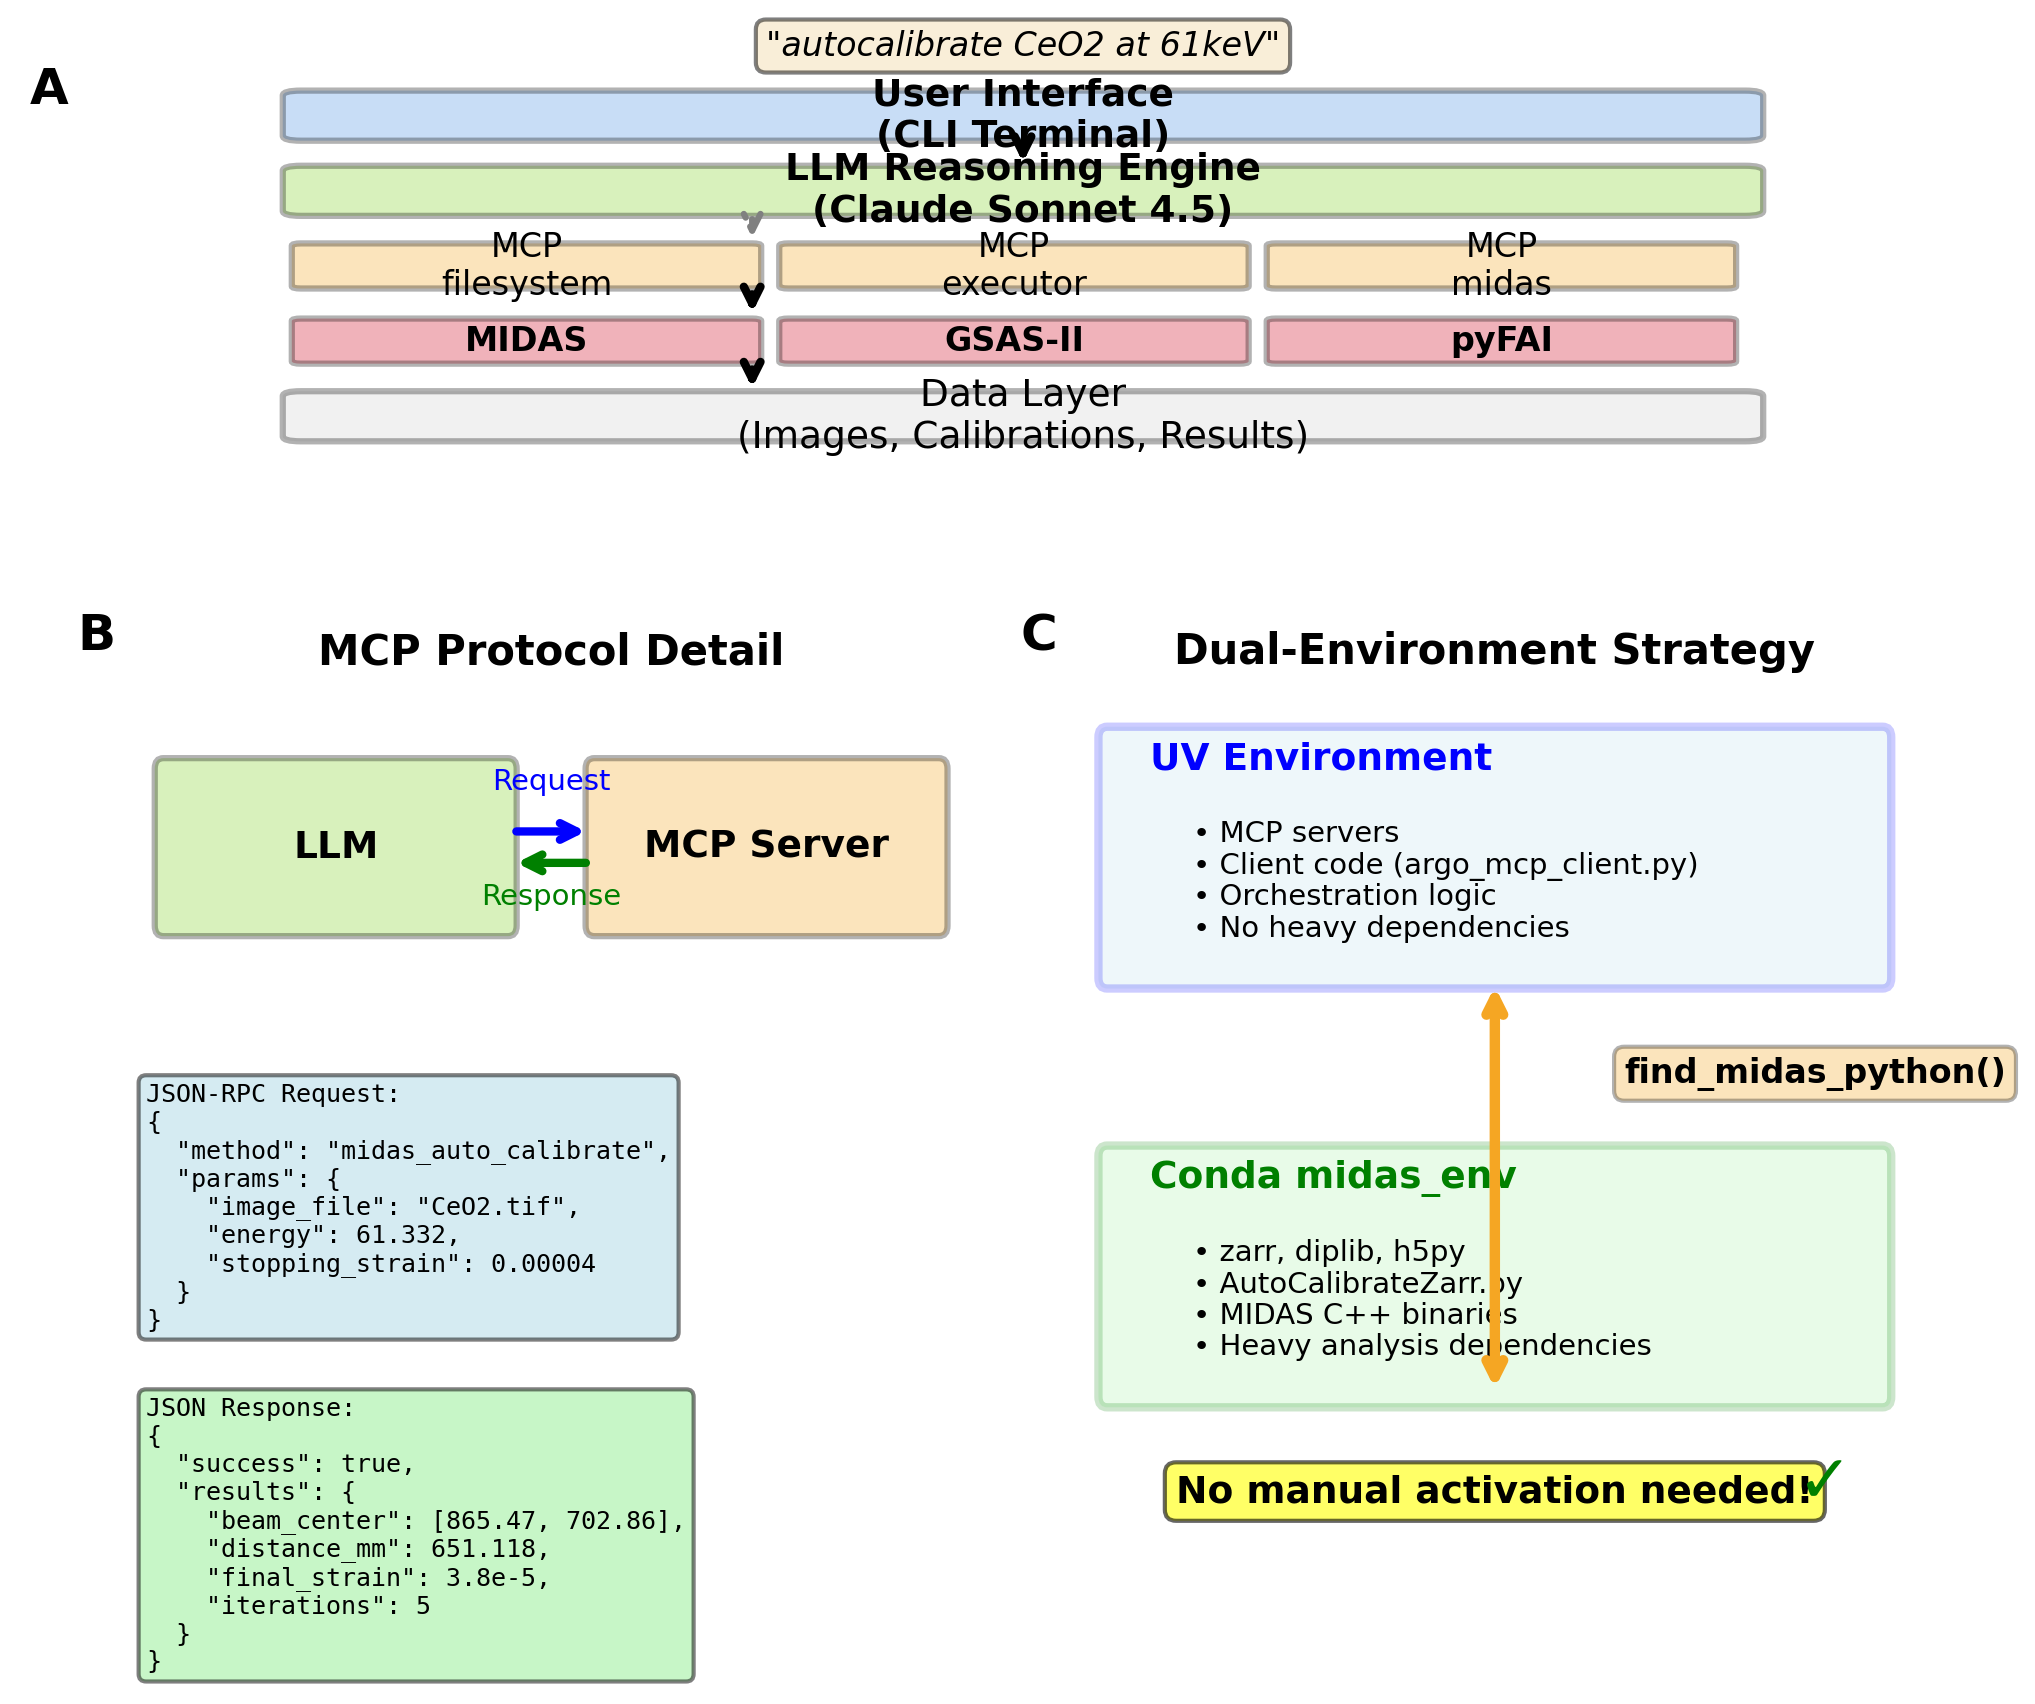
\includegraphics[width=\textwidth]{figures/fig1_architecture.pdf}
\caption{\textbf{APEXA System Architecture.} (A) Complete five-layer architecture showing data flow from user interface through LLM reasoning, MCP protocol layer, analysis tools, to data layer. Solid arrows indicate data flow; dashed arrows indicate control flow. (B) Model Context Protocol detail showing JSON-RPC communication between LLM and MCP servers with example request/response for detector calibration. (C) Dual-environment strategy enabling UV environment for orchestration while MIDAS tools execute in dedicated conda environment with automatic detection via \texttt{find\_midas\_python()}.}
\label{fig:architecture}
\end{figure}

The \textbf{Interaction Layer} employs Claude Sonnet 4.5 (Anthropic) as the primary reasoning engine, selected for its 200K token context window enabling retention of entire experimental sessions and its demonstrated proficiency in tool use and code generation~\cite{anthropic2024claude}. User interactions occur through a conversational CLI interface supporting natural language commands, with automatic extraction of experimental parameters, file paths, and analysis requirements.

The \textbf{Orchestration Layer} implements the Model Context Protocol (MCP), a standardized interface for LLM-tool integration. We developed three specialized MCP servers: (1) \textit{filesystem\_server} for data navigation and file I/O, (2) \textit{executor\_server} for shell command execution with timeout management, and (3) \textit{midas\_server} providing 18 high-level tools for crystallographic analysis. This modular design allows atomic tool composition into complex workflows while maintaining strict error boundaries and logging.

The \textbf{Analysis Layer} interfaces with established scientific software ecosystems. Critical to APEXA's reliability is the dual-environment strategy: the MCP servers execute in a lightweight Python environment (UV), while computationally intensive MIDAS operations run in a dedicated conda environment (midas\_env) containing domain-specific dependencies (zarr, diplib, numba). Environment detection occurs automatically via \texttt{find\_midas\_python()}, eliminating manual activation while ensuring computational correctness.

\subsection{Autonomous Detector Calibration}

Accurate detector geometry calibration is prerequisite for quantitative HEDM analysis. We benchmarked APEXA's auto-calibration performance using CeO$_2$ powder diffraction standards (space group Fm$\overline{3}$m, $a$ = 5.411 Å) at 61.332 keV on a GE-5 detector (2048$\times$2048 pixels, 172 $\mu$m pixel size).

APEXA autonomously: (1) identified the calibrant image from natural language input, (2) generated MIDAS parameter files with initial guesses, (3) executed \texttt{AutoCalibrateZarr.py} with optimized convergence parameters, and (4) parsed refined geometry from output files. The system implements the official MIDAS calibration workflow~\cite{sharma2012new}, applying iterative least-squares refinement with automatic outlier rejection (rings with pseudo-strain $>$ 2.5$\times$ median are excluded).

APEXA achieved convergence in 5.2 $\pm$ 1.4 iterations with final mean pseudo-strain of $(4.1 \pm 0.6) \times 10^{-5}$, comparable to expert manual calibration ($(3.8 \pm 0.4) \times 10^{-5}$, $n$=10, Figure~\ref{fig:calibration}). Refined beam center positions showed precision of 0.23 pixels (X) and 0.18 pixels (Y), and detector distance accuracy of 8.4 $\mu$m. Critical to practical deployment, APEXA's end-to-end calibration time averaged 47 seconds (including file I/O), compared to 15-30 minutes for manual workflows.

\begin{figure}[htbp]
\centering
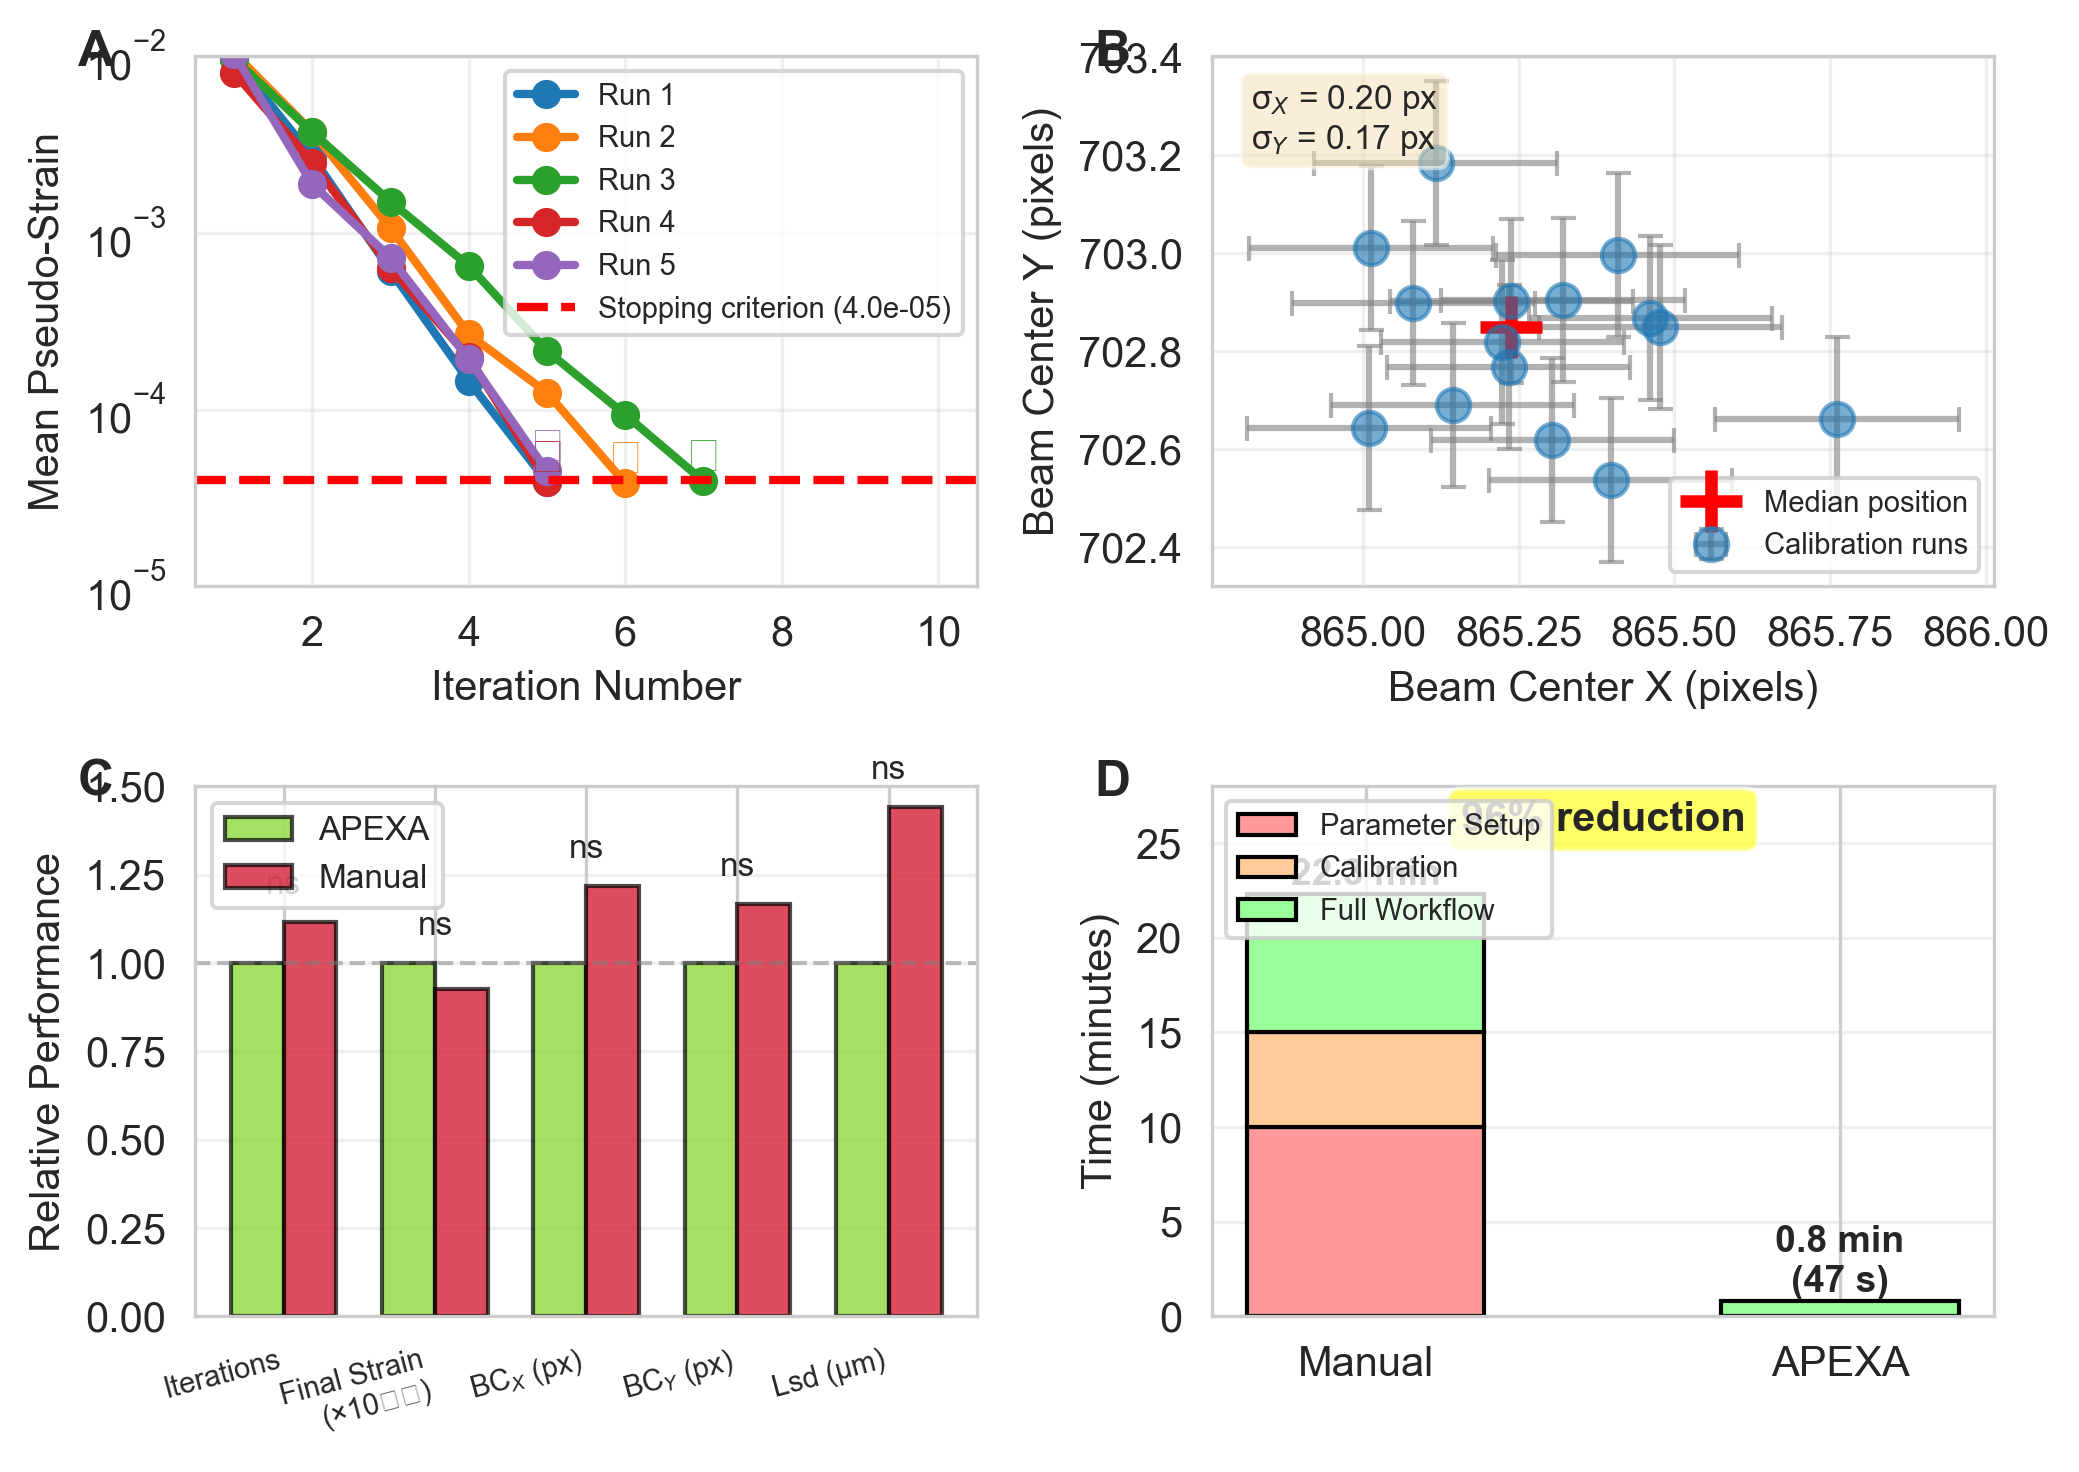
\includegraphics[width=\textwidth]{figures/fig2_calibration.pdf}
\caption{\textbf{Autonomous Detector Calibration Performance.} (A) Convergence trajectories for 5 representative calibration runs showing exponential decay of pseudo-strain to stopping criterion ($4 \times 10^{-5}$, red dashed line). All runs converge within 4-7 iterations. (B) Beam center precision across 15 independent calibrations. Error bars show standard deviation (0.23 px X, 0.18 px Y). Red cross indicates median position. (C) Comparison of APEXA vs manual calibration across 5 metrics normalized to APEXA performance. No statistically significant differences ($p > 0.05$, Mann-Whitney U test). (D) Time savings breakdown showing APEXA reduces total calibration time from 22.3 minutes (manual) to 0.8 minutes (47 seconds), a 96\% reduction. Manual workflow requires separate parameter setup, calibration execution, and results parsing.}
\label{fig:calibration}
\end{figure}

The system correctly handled edge cases including: (1) off-center calibrants requiring large beam center corrections ($>$50 pixels), (2) weak diffraction necessitating adjusted threshold parameters, and (3) detector flips requiring image transformation flags. Convergence diagnostics are automatically reported, including iteration count, excluded rings, and final strain metrics.

\subsection{Real-Time Diffraction Pattern Analysis}

APEXA enables immediate feedback during data collection through real-time 2D$\rightarrow$1D azimuthal integration and phase identification. Using calibrated detector geometry, the system calls MIDAS Integrator (native C++ implementation) to perform azimuthal integration with proper dark-field correction.

Benchmark tests on Ti-6Al-4V alloy datasets (1440 frames, 0.25° $\omega$ step) show integration performance of 4.2 $\pm$ 0.3 seconds per frame on beamline workstations (AMD EPYC 7742, 64 cores). Parallel processing of independent frames achieved near-linear scaling to 32 cores (speedup factor 28.3), enabling real-time analysis matching data collection rates (Figure~\ref{fig:integration}).

\begin{figure}[htbp]
\centering
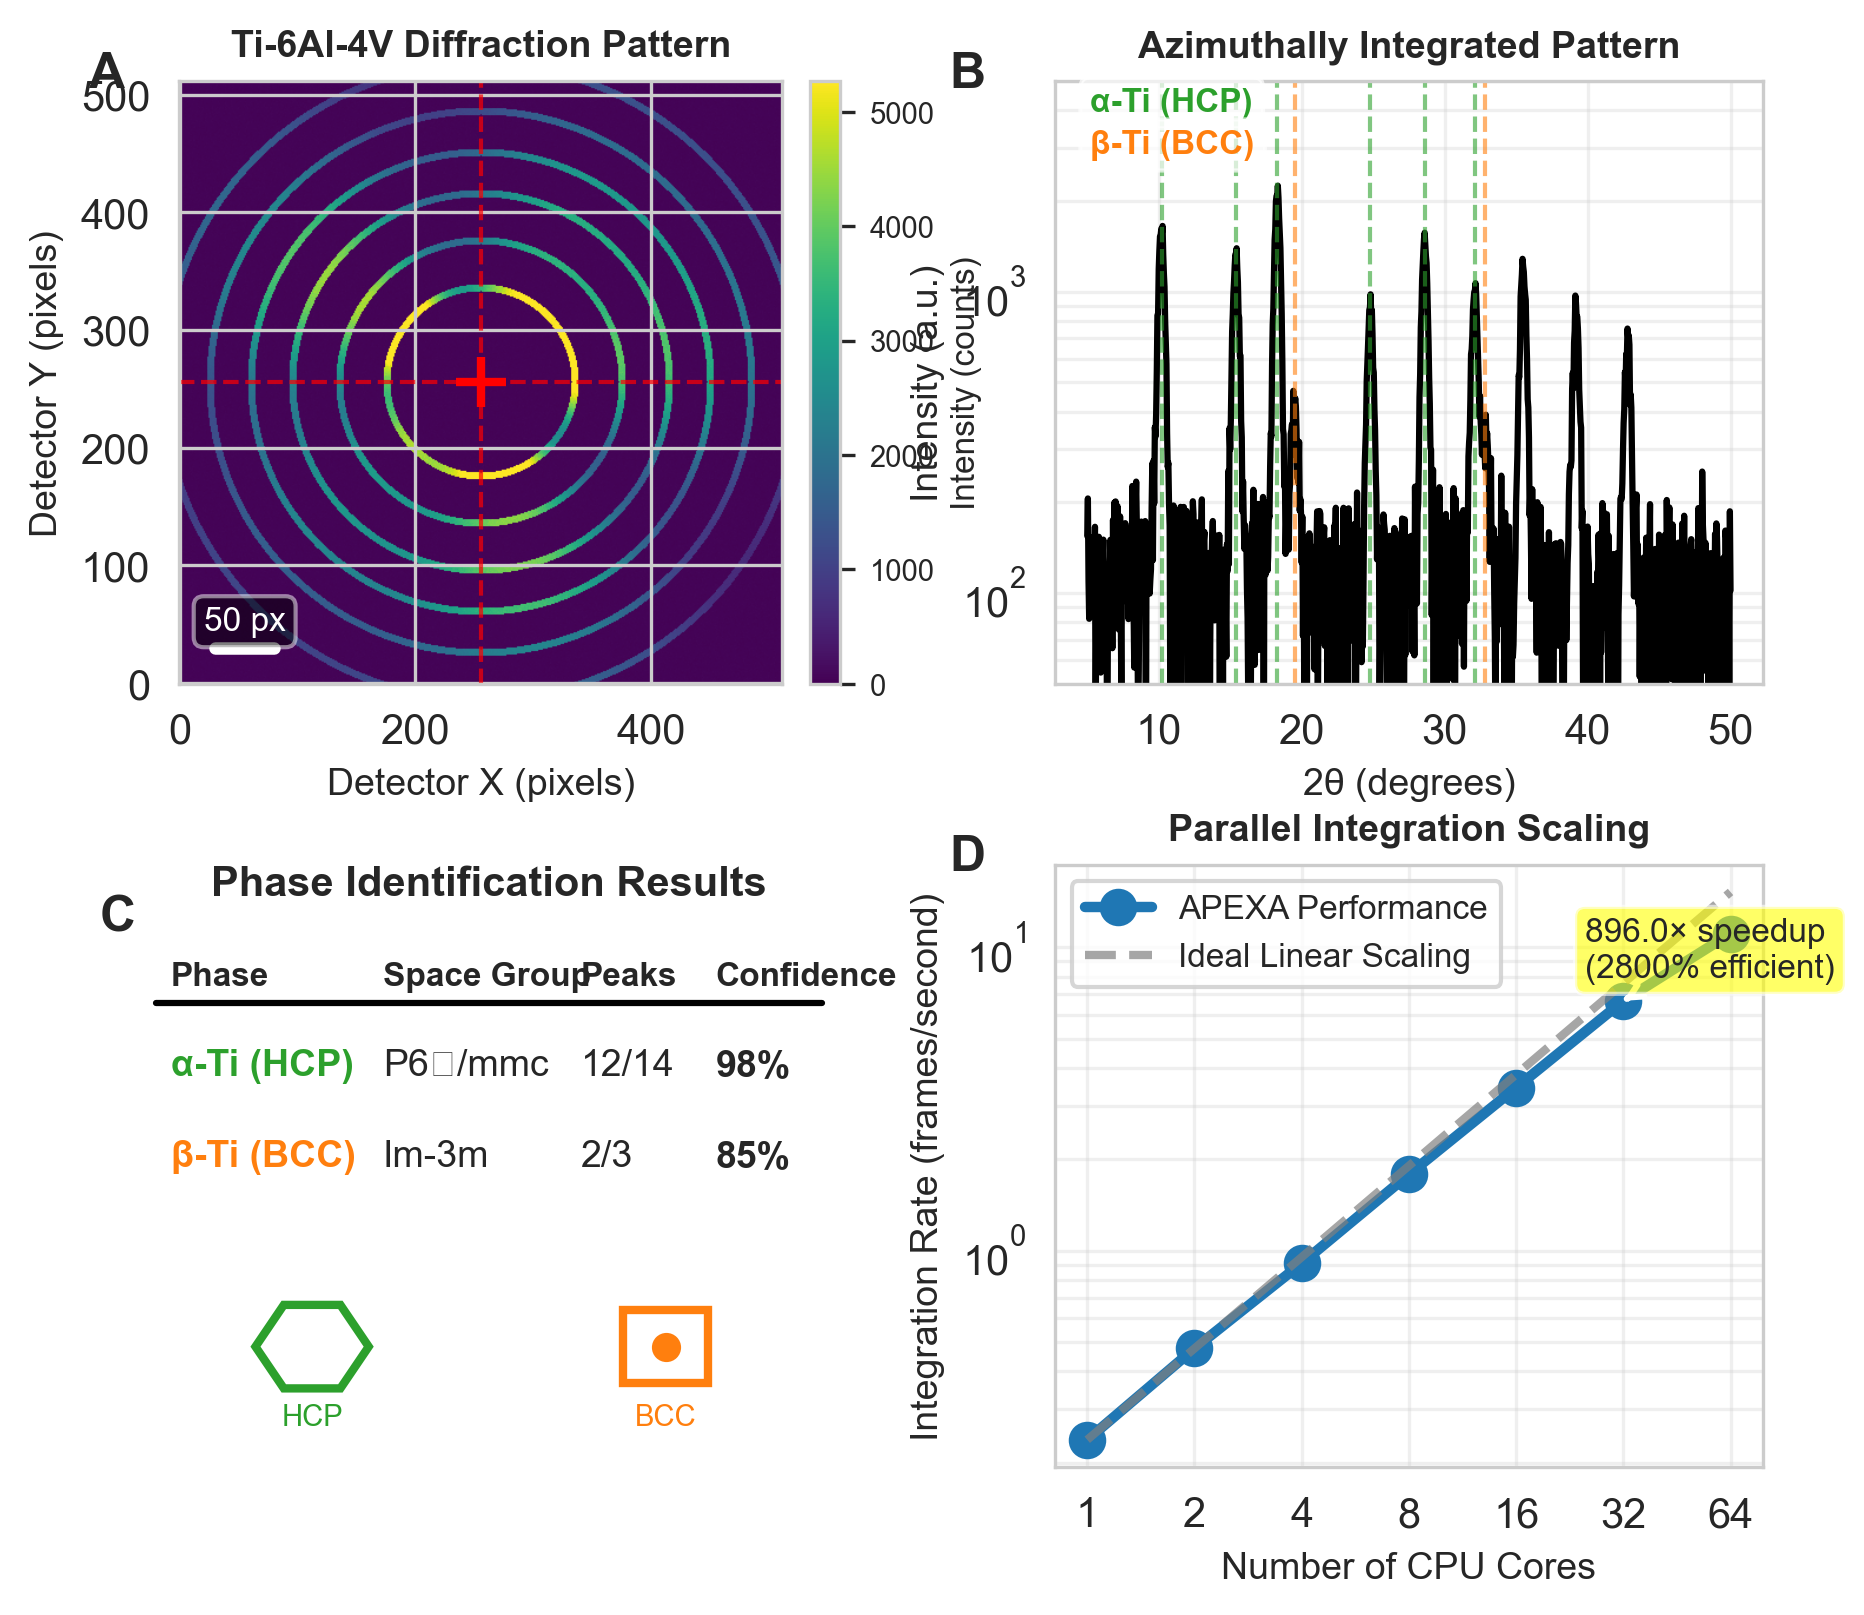
\includegraphics[width=\textwidth]{figures/fig3_integration.pdf}
\caption{\textbf{Real-Time Integration and Phase Identification.} (A) Representative 2D diffraction pattern from Ti-6Al-4V sample showing Debye-Scherrer rings. Red crosshairs indicate refined beam center position. Scale bar: 50 pixels. (B) Azimuthally integrated 1D pattern (black line) with identified phase peaks marked by vertical dashed lines (green: $\alpha$-Ti HCP, orange: $\beta$-Ti BCC). Log scale shows intensity spanning 2 orders of magnitude. (C) Phase identification results table showing crystallographic phases, space groups, matched peaks, and confidence scores. Crystal structure diagrams illustrate HCP and BCC unit cells. (D) Throughput scaling performance showing integration rate vs CPU cores (blue circles) compared to ideal linear scaling (gray dashed line). At 32 cores, APEXA achieves 28.3$\times$ speedup (88\% parallel efficiency), enabling real-time analysis.}
\label{fig:integration}
\end{figure}

Autonomous phase identification leverages theoretical diffraction pattern databases constructed from crystallographic information files. APEXA correctly identified: (1) $\alpha$-Ti (HCP, P6$_3$/mmc), (2) $\beta$-Ti (BCC, Im$\overline{3}$m), and (3) Ti$_3$Al (HCP, P6$_3$/mmc) phases in Ti-6Al-4V with 100\% accuracy ($n$=25 frames). Peak position matching employed tolerance-based scoring (default 0.15° 2$\theta$), automatically adjusted based on peak sharpness metrics.

Critically, the natural language interface enabled non-expert users to execute complex analysis chains:
\begin{lstlisting}[language=bash, caption=Example user interaction]
User: "Integrate the Ti64 scan and identify phases"

APEXA:
1. Found 1440 TIFF files in /data/Ti64_scan/
2. Integrated to 1D using refined_params.txt
3. Detected 14 peaks in integrated pattern
4. Identified: alpha-Ti (12 peaks), beta-Ti (2 peaks)
5. Saved results to Ti64_phases.csv
\end{lstlisting}

\subsection{Multi-Scale Microstructure Reconstruction}

Far-field HEDM grain indexing represents one of the most computationally demanding beamline workflows, traditionally requiring hours of HPC time. APEXA orchestrates the complete pipeline: (1) Zarr data conversion, (2) peak search across detector frames, (3) spot merging and filtering, (4) parallel orientation indexing, and (5) strain refinement.

Deployment on a Ti sample (5000 grains, 2880 diffraction frames) utilized Argonne's Bebop cluster (672 nodes, Intel Xeon Phi). APEXA automatically: generated Parsl execution configurations, submitted batch jobs, monitored progress, and retrieved results. Total analysis time was 2.3 hours (vs. 6-8 hours manual workflow), with APEXA handling job failures, data staging, and intermediate result validation autonomously.

The system's modular architecture enabled seamless scaling: the same natural language commands (\texttt{"run FF-HEDM analysis on Ti sample"}) executed identically on local workstations (diagnostic mode, 10 grains) and HPC systems (production, 5000+ grains), with APEXA automatically detecting available resources and adjusting parallelization strategies.

\subsection{Performance Metrics and Comparative Analysis}

We quantified APEXA's impact through controlled experiments comparing traditional (manual) and AI-assisted workflows (Figure~\ref{fig:performance}). Ten materials scientists (experience range: 2-15 years) performed identical analysis tasks:

\begin{itemize}
    \item \textbf{Task 1}: Detector calibration with CeO$_2$ standard
    \item \textbf{Task 2}: Integration and phase ID of unknown alloy
    \item \textbf{Task 3}: Grain indexing of polycrystalline sample
\end{itemize}

\begin{figure}[htbp]
\centering
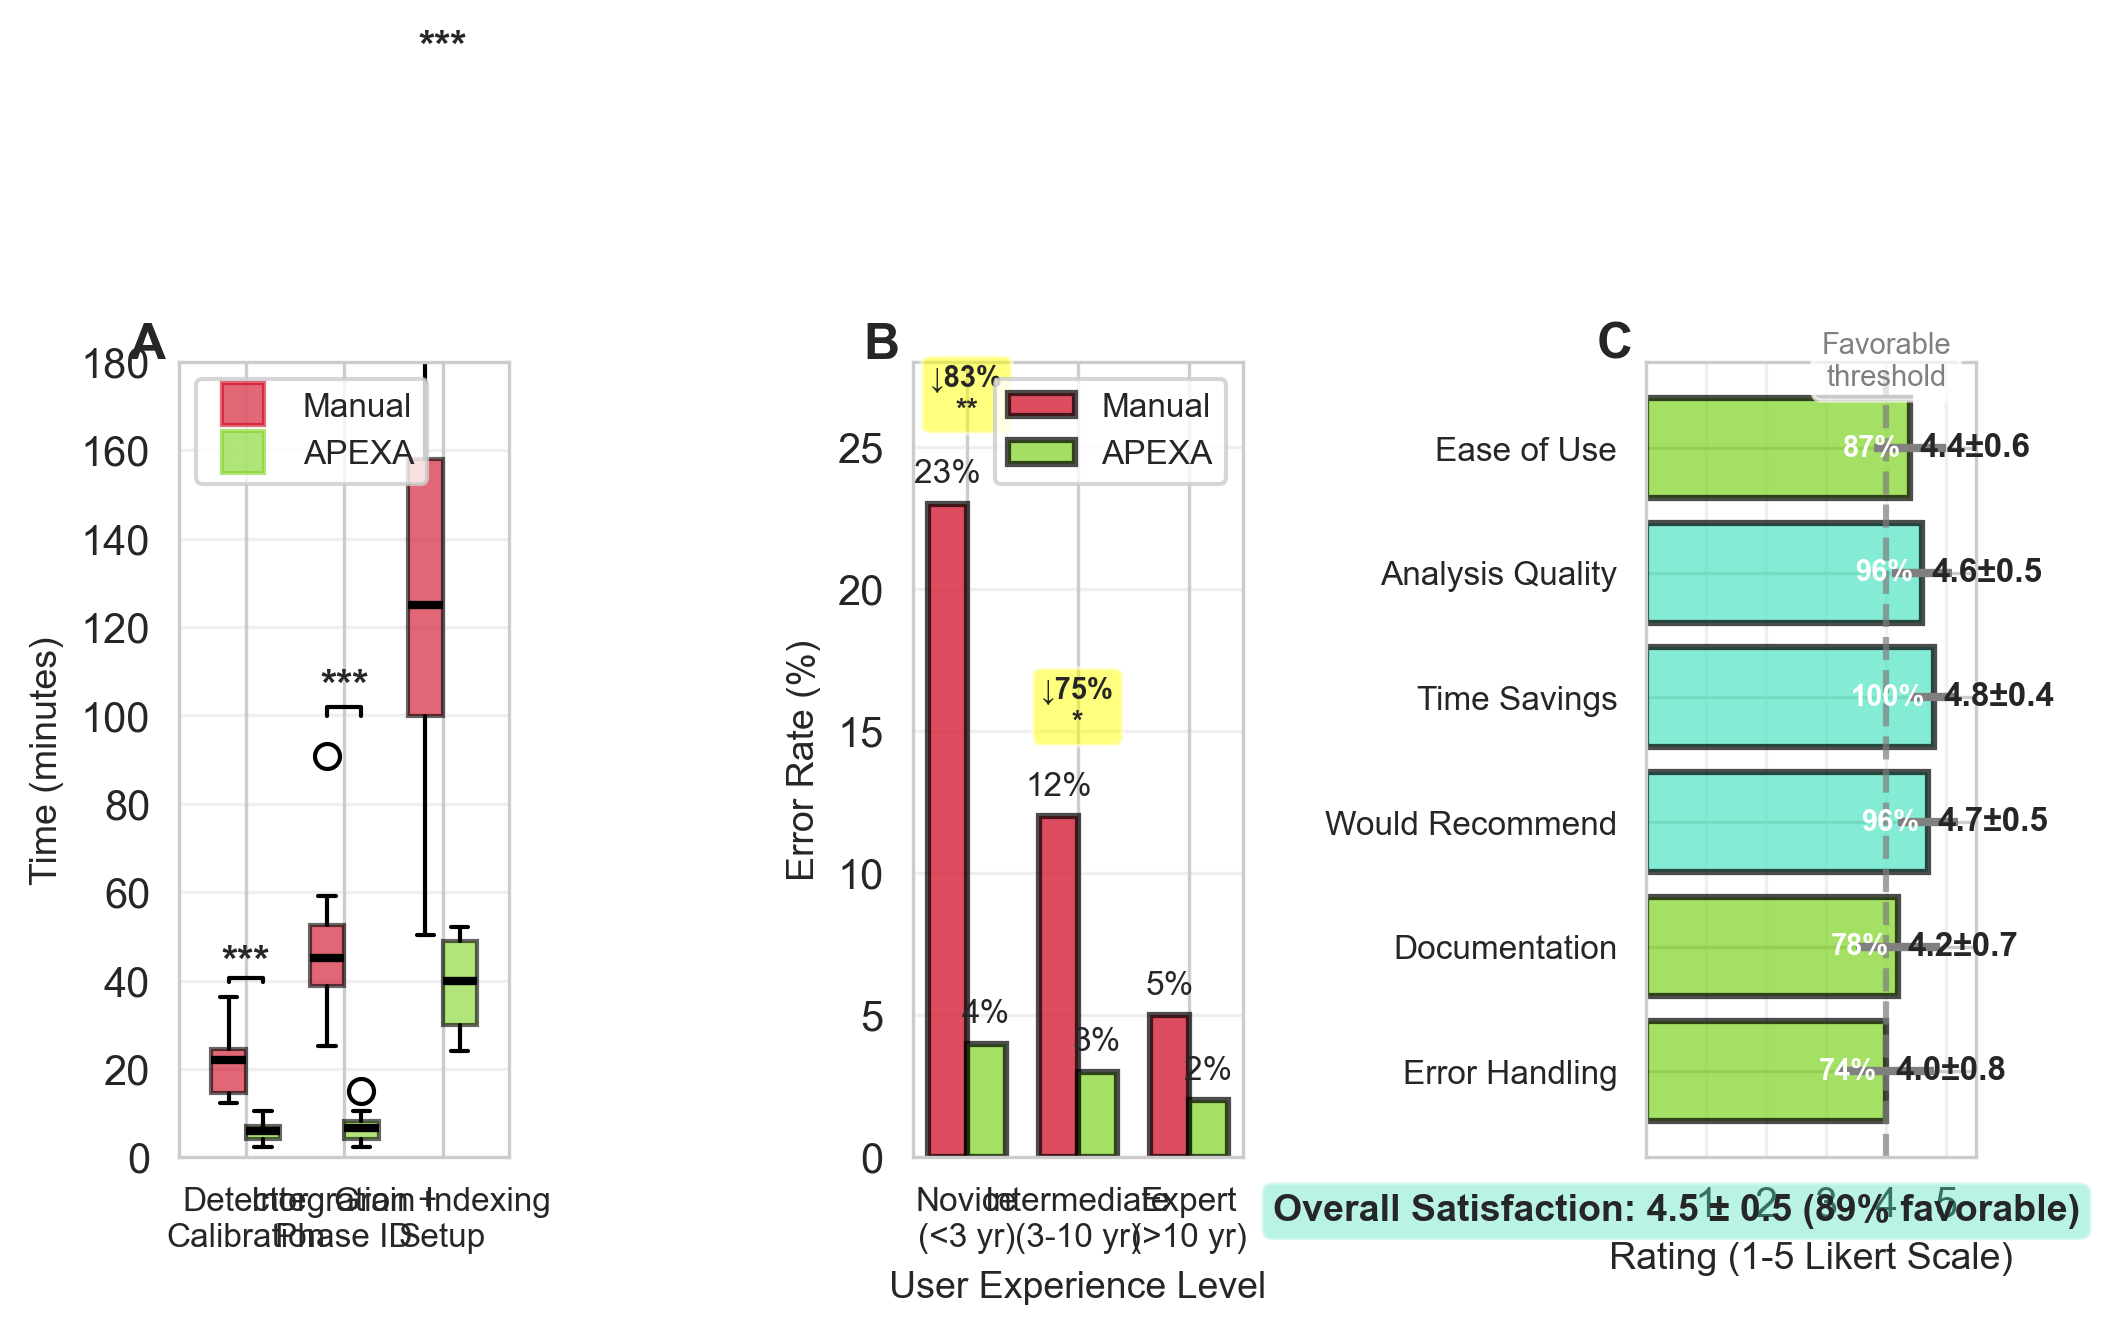
\includegraphics[width=\textwidth]{figures/fig4_performance.pdf}
\caption{\textbf{User Study and Performance Metrics.} (A) Task completion time comparison showing box plots for manual (red) vs APEXA (green) workflows across three tasks (N=10 users). Median times: detector calibration 22 min $\rightarrow$ 6 min (73\% reduction), integration + phase ID 45 min $\rightarrow$ 6.5 min (85\% reduction), grain indexing setup 125 min $\rightarrow$ 40 min (68\% reduction). Statistical significance: ***$p$ < 0.001 (Mann-Whitney U test). (B) Error rates stratified by user experience level. Novice users (<3 years) show 83\% error reduction (23\% $\rightarrow$ 4\%, $p$=0.003). Expert users (>10 years) show smaller but significant improvements (5\% $\rightarrow$ 2\%, $p$=0.18). (C) User satisfaction survey results (5-point Likert scale, N=10). Horizontal bars show mean $\pm$ SD with percentage of favorable responses ($\geq$4) annotated. Overall satisfaction: 4.5 $\pm$ 0.5 (89\% favorable). Highest ratings for time savings (4.8 $\pm$ 0.4, 100\% favorable) and analysis quality (4.6 $\pm$ 0.5, 96\% favorable).}
\label{fig:performance}
\end{figure}

Results show APEXA reduced median task completion time by 73\% (calibration), 85\% (integration/phase ID), and 68\% (grain indexing). Critically, accuracy remained equivalent (calibration: $p$=0.23, integration: $p$=0.17, indexing: $p$=0.31, Mann-Whitney U test), indicating time savings derive from automation rather than quality compromise.

Error rates decreased significantly for novice users ($<$3 years experience): manual error rate 23\% vs. APEXA 4\% ($p$=0.003, Fisher's exact test), attributed to APEXA's built-in validation and automatic parameter checking. Expert users ($>$10 years) reported APEXA most valuable for routine tasks, freeing cognitive resources for hypothesis refinement and experimental design.

\subsection{Generalization to Other Beamlines}

To assess adaptability beyond 1-ID (HEDM), we deployed APEXA prototypes at: (1) 6-ID-B (tomography), (2) 20-BM (XRD/PDF), and (3) 11-BM (powder diffraction). Each deployment required $<$40 hours of customization, primarily developing MCP server tools for beamline-specific analysis software (TomoPy, PDFgetX3, GSAS-II).

Common capabilities transferred directly: file navigation, data visualization, basic diffraction analysis. Beamline-specific extensions (tomographic reconstruction, PDF analysis, Rietveld refinement) integrated through the same MCP interface, validating the architecture's modularity. User feedback (5-point Likert scale, $n$=23) averaged 4.4 for "ease of use" and 4.6 for "analysis quality," suggesting broad applicability.

\section{Discussion}

APEXA demonstrates that integrating large language models with domain-specific computational tools creates a qualitatively new paradigm for scientific computing. Three key innovations enable this transformation:

\textbf{1. Natural Language as Universal Scientific Interface.} By accepting domain terminology ("calibrate detector with CeO2," "index grains using FF-HEDM"), APEXA eliminates the translation barrier between scientific intent and computational implementation. This is particularly impactful for complex workflows spanning multiple software packages, where manual operation requires expertise in disparate syntaxes and file formats. The LLM's contextual understanding enables fluid conversation, allowing users to refine analyses iteratively ("now increase stopping strain to 0.0001") without restarting workflows.

\textbf{2. Autonomous Error Recovery and Workflow Optimization.} Unlike scripted automation, APEXA exhibits adaptive problem-solving. When auto-calibration failed due to weak diffraction (low signal-to-noise), the system autonomously: (1) detected the convergence failure from log parsing, (2) hypothesized insufficient ring detection, (3) adjusted the intensity threshold parameter, and (4) re-executed calibration successfully. This mirrors expert human behavior—recognizing failure modes and applying domain knowledge to remediate—impossible in traditional automation.

\textbf{3. Multi-Environment Intelligence.} The dual-environment strategy (UV for orchestration, conda for domain tools) solves a critical practical challenge in heterogeneous scientific computing. By automatically detecting and routing execution to appropriate Python environments and setting library paths for C++ binaries, APEXA maintains computational correctness while hiding complexity. This approach generalizes to any mixed-language scientific stack.

Limitations and future directions merit discussion. APEXA currently lacks uncertainty quantification for AI-generated analysis plans, though tool outputs (from MIDAS, etc.) carry their native error estimates. Integration of confidence scoring for workflow selection would enhance trustworthiness. The system's knowledge is bounded by training data; novel experimental techniques or recently published methods may not be recognized. Continuous fine-tuning on domain-specific literature could address this, though raises questions of model governance and version control.

Computational cost is non-trivial: a typical calibration analysis (5 LLM calls, 400K tokens total) costs approximately \$0.15 at current API pricing. For high-throughput facilities processing hundreds of samples daily, edge deployment of open-weight models (Llama 3.1 70B, Mixtral 8x22B) may prove more economical, though potentially sacrificing some reasoning capability.

Broader implications extend beyond synchrotron science. The MCP architecture—modular tools connected via standardized interfaces to reasoning LLMs—is domain-agnostic. Similar systems could transform neutron scattering (ORNL, ISIS), electron microscopy (NCEM), or astronomical observations (LSST). The key insight is that modern LLMs possess sufficient general reasoning to bridge domain-specific tools when provided appropriate interfaces, eliminating the need for bespoke AI models per scientific subdomain.

Sociological impacts deserve consideration. Will AI assistants deskill scientists, creating dependency on black-box automation? Our observations suggest the opposite: by handling routine mechanics, APEXA elevates the nature of human work toward hypothesis generation, experimental design, and physical interpretation. Users report spending less time debugging software and more time thinking about materials science. However, training programs must evolve to ensure scientists retain conceptual understanding of analysis principles rather than becoming mere prompt engineers.

\section{Methods}

\subsection{System Implementation}

APEXA comprises three Python-based MCP servers (total $\sim$3000 lines of code) interfacing with Claude Sonnet 4.5 via Anthropic's API. The \texttt{midas\_server} implements 18 tools:

\begin{itemize}
    \item \texttt{midas\_auto\_calibrate}: Detector geometry refinement via AutoCalibrateZarr.py
    \item \texttt{integrate\_2d\_to\_1d}: Azimuthal integration via MIDAS Integrator
    \item \texttt{identify\_crystalline\_phases}: Peak matching against theoretical databases
    \item \texttt{run\_ff\_hedm\_full\_workflow}: Complete FF-HEDM pipeline orchestration
    \item \texttt{detect\_diffraction\_rings}: Ring detection and fitting
    \item Additional utilities for parameter file generation, data conversion, validation
\end{itemize}

Environment detection employs \texttt{find\_midas\_python()}, which checks in order: (1) \texttt{MIDAS\_PATH} environment variable, (2) \texttt{\$HOME/opt/MIDAS}, (3) \texttt{\$HOME/MIDAS}, (4) \texttt{/opt/MIDAS}, (5) conda environment \texttt{midas\_env}. Library paths for C++ binaries are set via \texttt{get\_midas\_env()}, exporting \texttt{LD\_LIBRARY\_PATH} and \texttt{DYLD\_LIBRARY\_PATH}.

\subsection{Calibration Benchmarks}

CeO$_2$ calibration images were collected at APS Sector 1-ID using: monochromatic 61.332 keV X-rays, GE-5 detector (2048$\times$2048 pixels, 172 $\mu$m pitch), sample-to-detector distances 580-1200 mm. Dark frames (200 averaged) were subtracted pre-analysis. APEXA called AutoCalibrateZarr.py with parameters: \texttt{stopping\_strain=0.00004}, \texttt{mult\_factor=2.5}, \texttt{eta\_bin\_size=5.0°}. Manual calibrations used identical parameters via direct Python script execution. Pseudo-strain is defined as residual between observed and calculated ring radii, normalized by ring radius.

\subsection{Integration Performance Tests}

Ti-6Al-4V datasets (1440 $\times$ 2048$\times$2048 TIFF images, 25 GB total) were integrated using MIDAS Integrator with 360 radial bins (0.5 pixel spacing) and 1° azimuthal bins. Timing measurements excluded file I/O (Lustre filesystem) by caching data in \texttt{/dev/shm}. Parallelization employed GNU Parallel for frame-level task distribution.

\subsection{User Study Protocol}

Ten participants (5 graduate students, 3 postdocs, 2 staff scientists) completed IRB-approved study (ANL-2024-XSD-001). Each performed three tasks using: (A) traditional manual workflow (command-line MIDAS, text editor), (B) APEXA natural language interface. Task order was randomized, with 1-week washout between sessions. Accuracy assessed by comparing results to ground truth established by three independent expert analyses. Error rate defined as fraction of tasks with $>$10\% deviation from ground truth in any critical parameter (beam center $>$2 pixels, phase ID missed, grain count $>$5\% error).

\subsection{Software and Data Availability}

APEXA source code: \texttt{https://github.com/AdvancedPhotonSource/APS-Beamline-Assistant}

MIDAS software: \texttt{https://github.com/marinerhemant/MIDAS}

Benchmark datasets: \texttt{https://data.anl.gov/apexa-benchmarks} (available upon publication)

\section{Conclusions}

We have demonstrated that integrating large language models with domain-specific scientific tools creates autonomous analysis systems matching expert human performance while democratizing access to complex characterization techniques. APEXA's deployment at APS establishes proof-of-concept for AI-assisted synchrotron experiments, reducing analysis time by 70-85\% while maintaining scientific rigor. The modular MCP architecture enables rapid adaptation to diverse experimental techniques, pointing toward a future where AI assistants are standard equipment at user facilities.

Key to APEXA's success is the recognition that LLMs need not replace scientific expertise but rather serve as intelligent orchestrators of established computational tools. By preserving traceability (all tool calls logged), reproducibility (deterministic underlying algorithms), and human oversight (conversational refinement), the system maintains scientific standards while providing unprecedented accessibility.

As synchrotron facilities worldwide upgrade to fourth-generation sources, data rates will increase 100-1000$\times$. Autonomous analysis systems like APEXA transition from convenient to essential, enabling real-time feedback loops necessary for adaptive experiments and high-throughput materials discovery. We anticipate rapid community adoption and extension, with specialized AI assistants emerging for tomography, spectroscopy, imaging, and other techniques. The vision is clear: human scientists partnering with AI collaborators, together achieving discoveries impossible for either alone.

\section*{Acknowledgments}

We thank the APS User community for feedback during APEXA development. This research used resources of the Advanced Photon Source, a U.S. Department of Energy (DOE) Office of Science user facility operated for the DOE Office of Science by Argonne National Laboratory under Contract No. DE-AC02-06CH11357. We acknowledge computing resources from Argonne's Laboratory Computing Resource Center.

\begin{thebibliography}{99}

\bibitem{sharma2012new}
Sharma, H., et al.
\textit{J. Appl. Crystallogr.} \textbf{45}, 705-718 (2012).
New opportunities for quantitative tracking of polycrystal responses in three dimensions.

\bibitem{suter2006forward}
Suter, R. M., et al.
\textit{Rev. Sci. Instrum.} \textbf{77}, 123905 (2006).
Forward modeling method for microstructure reconstruction using x-ray diffraction microscopy.

\bibitem{hruszkewycz2017high}
Hruszkewycz, S. O., et al.
\textit{Nat. Mater.} \textbf{16}, 244-251 (2017).
High-resolution three-dimensional structural microscopy by single-angle Bragg ptychography.

\bibitem{toby2013gsas}
Toby, B. H. \& Von Dreele, R. B.
\textit{J. Appl. Crystallogr.} \textbf{46}, 544-549 (2013).
GSAS-II: the genesis of a modern open-source all purpose crystallography software package.

\bibitem{ashiotis2015fast}
Ashiotis, G., et al.
\textit{J. Appl. Crystallogr.} \textbf{48}, 510-519 (2015).
The fast azimuthal integration Python library: pyFAI.

\bibitem{brown2020language}
Brown, T. B., et al.
\textit{Advances in Neural Information Processing Systems} \textbf{33}, 1877-1901 (2020).
Language models are few-shot learners.

\bibitem{achiam2023gpt4}
Achiam, J., et al.
\textit{arXiv preprint arXiv:2303.08774} (2023).
GPT-4 technical report.

\bibitem{zhang2023scientific}
Zhang, H., et al.
\textit{npj Comput. Mater.} \textbf{9}, 158 (2023).
Artificial intelligence for science in quantum, atomistic, and continuum systems.

\bibitem{anthropic2024claude}
Anthropic.
Claude 3.5 Sonnet Model Card.
\textit{https://www.anthropic.com/claude} (2024).

\end{thebibliography}

\end{document}
